\documentclass[pdftex,a4paper,11pt]{article}
\usepackage[utf8]{inputenc}

\usepackage{amssymb}
\usepackage{graphicx}
\usepackage{color}
\usepackage{verbatim}
\usepackage{amsthm} 
\usepackage{amsmath}
\usepackage{here}
\usepackage{epstopdf}

%opening
\title{Advanced topics in Machine Learning. \\ Concept of the solution of the programming assignment}
\author{ Team Chanjo. \\ Johannes Jendersie, Anton Niadzelka }

\begin{document}

\maketitle

\section{Challenge decription}
The challenge’s objective is easily described: Create a recommender system for first names! Given a set of names for which a user has shown interest in, the recommender should provide suggestions for further names for that user. The recommender’s quality will be assessed on an evaluation data set. Thus, the task can be considered a standard item recommendation task.

\section{Solution}

We received data about user activities from nameling.net website. Data consists of 515,848 activities made by 60,922 users. Our idea is to assign to each activity corresponding rating. The most explicit user expression will be ranked higher. \textit{ENTER SEARCH} will receive the highest rank, as  the evaluation is restricted only to this activity and all other activities are biased towards the lists of names which were displayed. 


So, afterwards we will get a table where for each name we will have some user rating or nothing. It is not possible to store the whole table on a usual laptop RAM, as the number of user names is too high. Moreover, the table is sparse as we have less than 10 activities in average pro user. So, we store only existing ratings for each user with the index number of the corresponding name.

The recommendation approach we are going to use is based on a model (\ref{1}) described in the book Recommender Systems Handbook \cite{1}. 

\begin{equation} \label{1} \hat{r}_{u i} = \mu + b_u + b_i + q^T _i \left( | R(U) |^{ - \frac{1}{2}} \sum_{j \in R(u) } (r_{u j} - b_{u j}) x_j + y_j ) \right) \text{, where} \end{equation}
\begin{center} $  \mu \text{ - average overl all table  ,}  $ \end{center}
\begin{center} $   R(u) \text{ - set that contains all items rated by user u,} $ \end{center}
\begin{center} $ b_u $ and $ b_i $ indicate the observed deviations of user u and item i, respectively, from the average.
 \end{center}
\begin{center} $  b_{u i} = \mu + b_u + b_i $ \end{center}
\begin{center} $  y_j $  - factors used to characterize users \\ based on the set of items they rated.   \end{center}
\begin{center} $  x_j $ - factors used to characterize items \\ based on the set of items they rated.  \end{center}
\begin{center} For a given item i, the elements of $ q_i $ measure the extent \\ to which the item possesses those factors, positive or negative. \end{center}

The factors mentioned above are obtained using a singular value decomposition (SVD) of an initial matix, as SVD maps both users and items to a joint latent factor space of dimensionality $ f $. As stated in book \cite{1} the latent space tries to explain ratings by characterizing both products and users on factors automatically inferred from user feedback. Usual SVD algorithms are not easily applicable in our case, as we have a really huge sparse matrix. Unfortunately there is no optimized Java library to do this. So, we are going to use the algorithm described in \cite{2} in chapter 4.3 to compute $q_j$.

We are going to try to modify the algorithm such that we obtain $x_j$ and $y_j$. In case that we do not achieve an initialization of these we will use the following method as fall back.
\begin{equation} \label{1.2} \hat{r}_{u i} = \mu + b_u + b_i + p^T _u q_i \end{equation}
In this method item-item and user-user relationships are not expressed explicit. To compensate the loss of information the rank $f$ has to be increased by a factor of 2.

\subsection{Learning}

The values $b_u$ and $b_i$ has to be learned after the initialization. During that learning $x_j$ and $y_j$ will be adapted too.
\begin{figure}[H]
	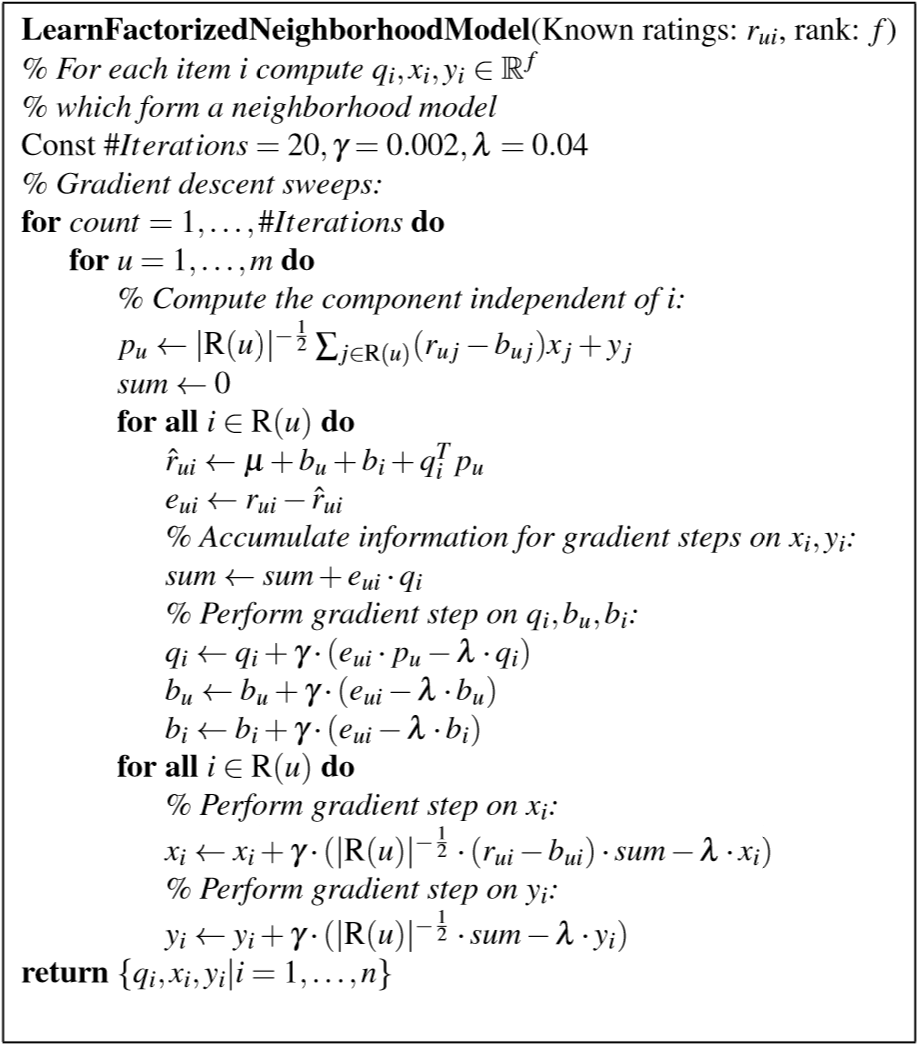
\includegraphics[width=1\textwidth]{Algorithm.png}
	\caption{Learning algorithm from \cite{1}}
	\label{fig:LearningAlg}
\end{figure}


\section{Evaluation}

The quality of the result will be measured by the root mean squared error (\ref{2}).
 
\begin{equation} \label{2} \sqrt{ \sum_{(u,i) \in TestSet} (r_{u i} - \hat{r}_{u i} ) ^2 / \left| TestSet \right| } \end{equation}

We have a few parameters that have to be tuned. These are initial ratings for each action and the number of latent factors $ f $. For that we are going to cross validate our model with different values of these parameters and afterwards choose the one with the best result. 

\section{Work Plan}

\begin{figure}[ht]
	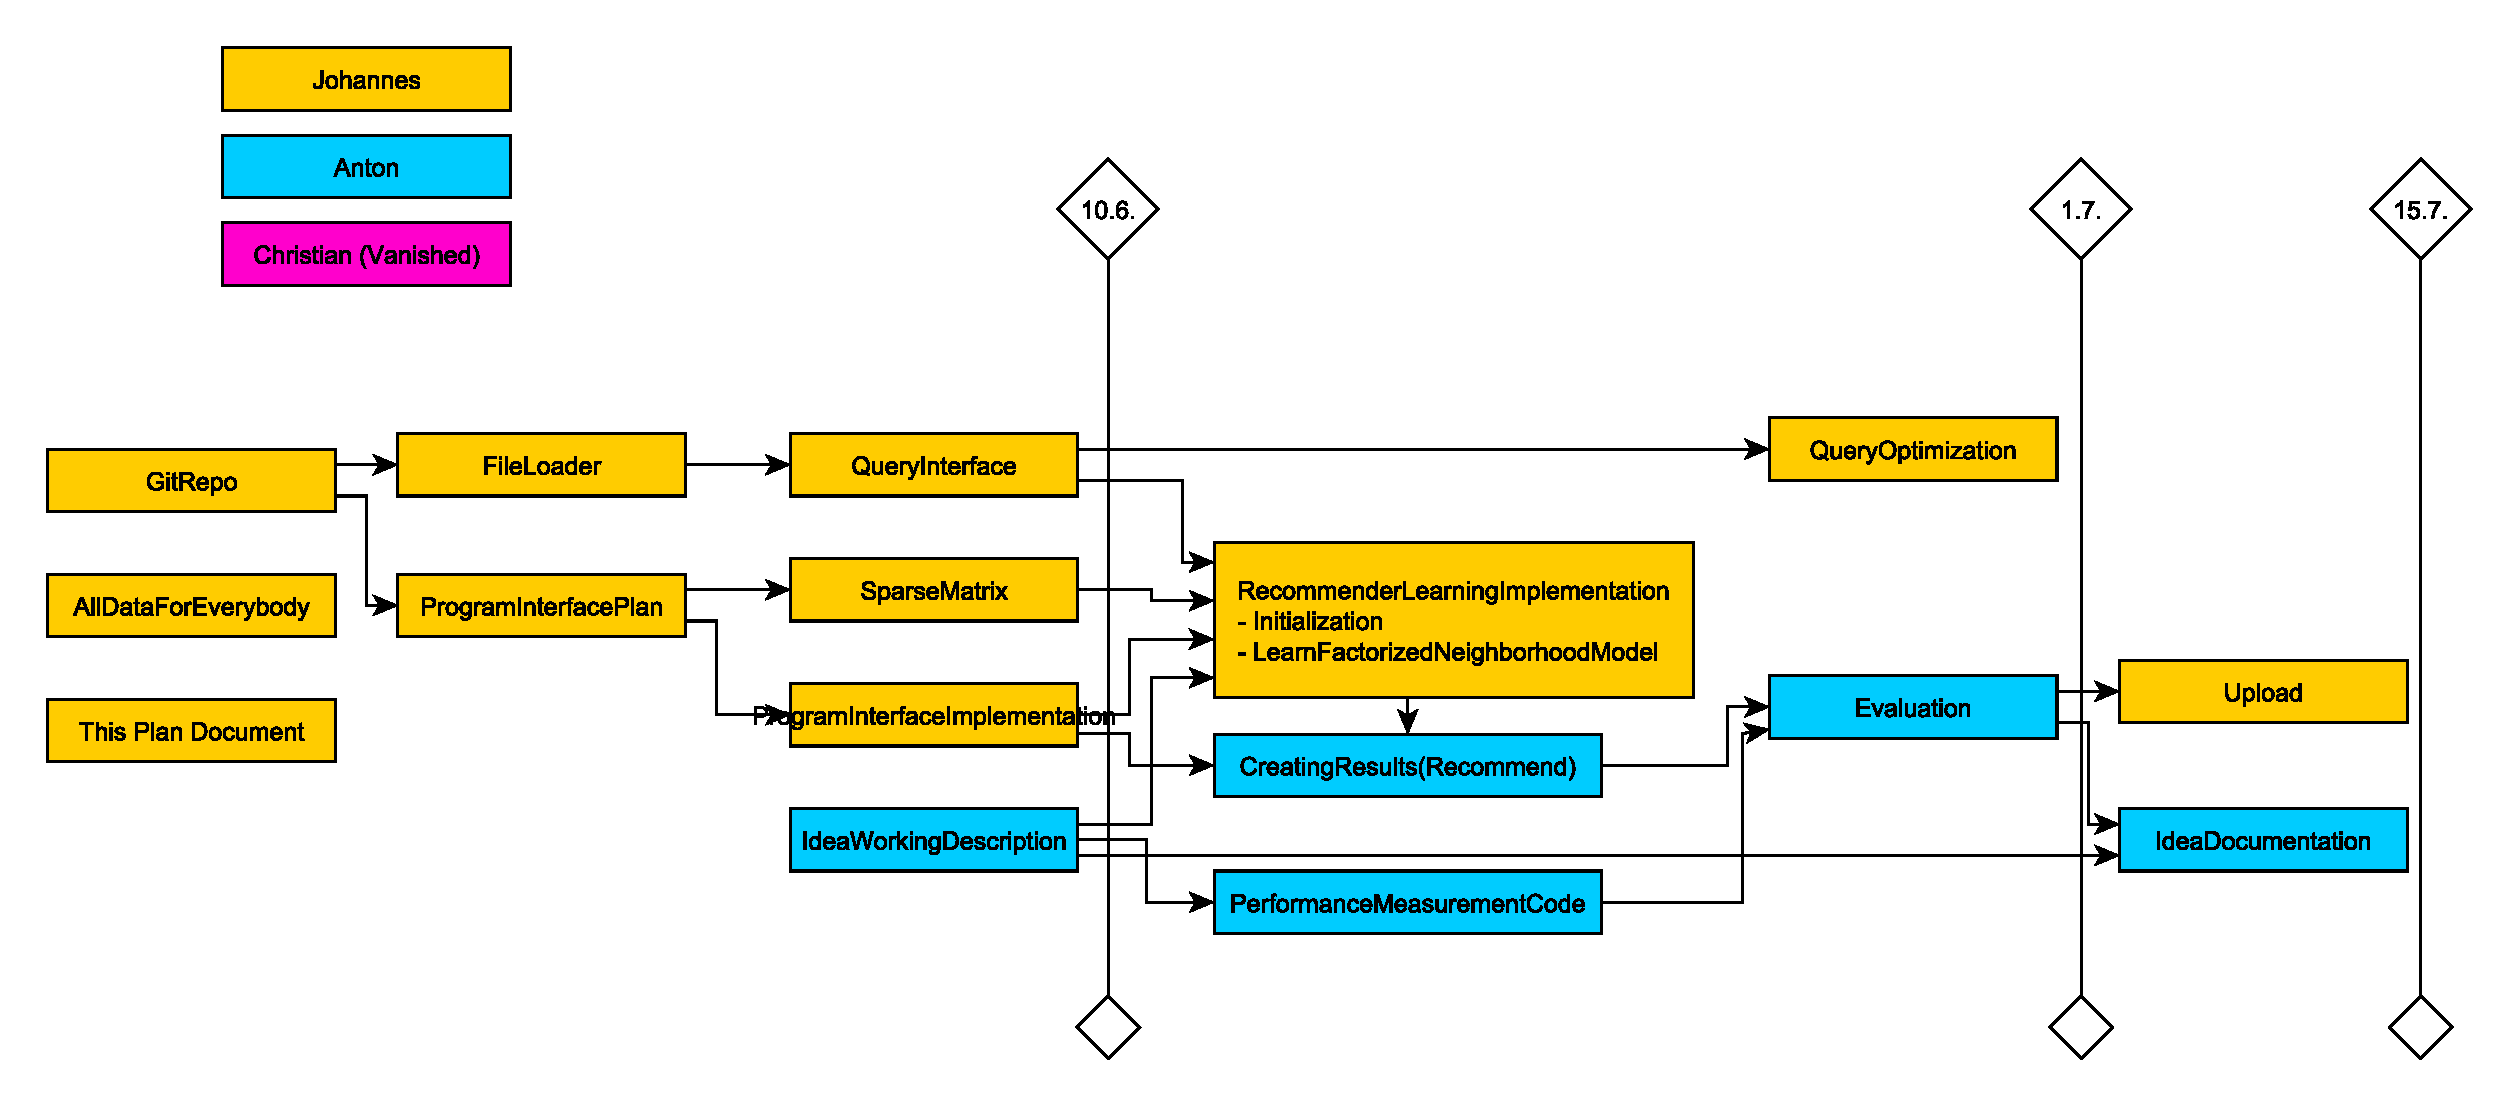
\includegraphics[width=1\textwidth]{WorkPlan.eps}
	\caption{Graphical plan representation with dependencies and deadlines}
	\label{fig:WP}
\end{figure}

Johannes Jendersie:

\begin{enumerate}
\item Team work organisation,
\item Program Interface,
\item Sparse Matrix,
\item Recommender Algorithm implementation.
\item Query Interface
\end{enumerate}
Anton Niadzelka:

\begin{enumerate}
\item Idea Description, 
\item Documentation,
\item Evaluation,
\item Performance Measurement implementation,
\item Recommendation creation
\end{enumerate}

\begin{thebibliography}{99}
\bibitem{1} Recommender Systems Handbook by Ricci, F.; Rokach, L.; Shapira, B.; Kantor, P.B. 2011, XXIX, Springer,  Chapter 5
\bibitem{2}  Modeling Relationships at Multiple Scales to Im-prove Accuracy of Large Recommender Systems, Bell, R.M., Koren, Y., and Volinsky, C., Proc. 13th ACM SIGKDD International
Conference on Knowledge Discovery and Data Mining, 2007.
\end{thebibliography}
\nocite{*}
\bibliographystyle{cell}
\bibliography{literature}

\end{document}